\documentclass[12pt]{article}
\usepackage[top=1in, bottom=1in, left=.75in, right=.75in]{geometry}
\usepackage{amsmath}


%\usepackage{draftwatermark}
%\SetWatermarkText{draft}
%\SetWatermarkScale{1}
%\SetWatermarkLightness{.9}

%\usepackage[]{enumitem}
\usepackage{enumerate}
\usepackage{fancyhdr}
%\usepackage{graphicx, xcolor, setspace, adjustbox}
\usepackage{txfonts}
\usepackage{multicol,coordsys,pgfplots}
\usepackage[scaled=0.86]{helvet}
\renewcommand{\emph}[1]{\textsf{\textbf{#1}}}
\usepackage{anyfontsize}
% \usepackage{times}
% \usepackage[lf]{MinionPro}
\usepackage{tikz,pgfplots}
%\def\degC{{}^\circ{\rm C}}
\def\ra{\rightarrow}
\usetikzlibrary{calc,arrows.meta, shapes, angles, quotes}
\pgfplotsset{compat = newest}
\newcommand{\blank}[1]{\rule{#1}{0.75pt}}

\pgfplotsset{my style/.append style={axis x line=middle, axis y line=
middle, xlabel={$x$}, ylabel={$y$}}}


%\usepackage{draftwatermark}
%\SetWatermarkText{Draft}
%\DraftwatermarkOptions{color={[gray]{.9}}}
%\SetWatermarkScale{1.5}

%axis equal

%yticklabels={,,} , xticklabels={,,}

% \setmainfont{Times}
% \def\sansfont{Lucida Grande Bold}
\parindent 0pt
\parskip 4pt
\pagestyle{fancy}
\fancyfoot[C]{\emph{\thepage}}
\fancyfoot[R]{v1}
\fancyhead[L]{\ifnum \value{page} > 1\relax\emph{Math F251X Calculus I: Final Exam}\fi}
\fancyhead[R]{\ifnum \value{page} > 1\relax\emph{Spring 2025}\fi}
\headheight 15pt
\renewcommand{\headrulewidth}{0pt}
\renewcommand{\footrulewidth}{0pt}
\let\ds\displaystyle
\def\continued{{\emph {Continued....}}}
\def\continuing{{\emph {Problem \arabic{probcount} continued....}}\par\vskip 4pt}


\newcounter{probcount}
\newcounter{subprobcount}
\newcounter{subsubprobcount}
\newcommand{\thesubproblem}{\emph{\alph{subprobcount}.}}
\newcommand{\thesubsubproblem}{\emph{\roman{subsubprobcount}.}}
\def\problem#1{\setcounter{subprobcount}{0}%
\addtocounter{probcount}{1}{\emph{\arabic{probcount}.\hskip 1em(#1)}}\par}
\def\subproblem#1{\par\hangindent=1em\hangafter=0{%
\addtocounter{subprobcount}{1}\thesubproblem\emph{#1}\hskip 1em}}
\def\subsubproblem#1{\par\hangindent=1em\hangafter=0{%
\addtocounter{subsubprobcount}{1}\thesubsubproblem\emph{#1}\hskip 1em}}
\def\probskip{\vskip 10pt}
\def\medprobskip{\vskip 2in}
\def\subprobskip{\vskip 45pt}
\def\bigprobskip{\vskip 4in}


\newenvironment{subproblems}{%
\begin{enumerate}%
\setcounter{enumi}{\value{subprobcount}}%
\renewcommand{\theenumi}{\emph{\alph{enumi}}}}%
{\setcounter{subprobcount}{\value{enumi}}\end{enumerate}}

\newenvironment{subsubproblems}{%
\begin{enumerate}%
\setcounter{enumi}{\value{subsubprobcount}}%
\renewcommand{\theenumi}{\emph{\roman{enumi}}}}%
{\setcounter{subprobcount}{\value{enumi}}\end{enumerate}}


\newcommand{\be}{\begin{enumerate}}
\newcommand{\ee}{\end{enumerate}}


\begin{document}

{\emph{\fontsize{26}{28}\selectfont Spring 2025 \hfill
\hfill Math F251X}}

\begin{center}
{\emph{\fontsize{32}{36}\selectfont Calculus I: Final Exam}}
\end{center}
\vskip 1.cm

\strut\vtop{\halign{\emph#\hskip 0.5em\hfil&#\hbox to 2in{\hrulefill}\cr
\emph{\fontsize{18}{22}\selectfont Name:}&\cr
\noalign{\vskip 10pt}
%\emph{\fontsize{18}{22}\selectfont Student Id:}&\cr
%\noalign{\vskip 10pt}
%\emph{\fontsize{18}{22}\selectfont Calculator Model:}&\cr
}}
\hfill
\vtop{\halign{\emph{\fontsize{18}{22}\selectfont #}\hfil& \emph{\fontsize{18}{22}\selectfont\hskip 0.5ex $\square$ #}\hfil\cr
Section: & 9:15 (James Gossell)\cr
\noalign{\vskip 4pt}
         & 11:45 (Kevin Meek)\cr
\noalign{\vskip 4pt}
         & Online (Deven Barnett)\cr}}
%
%\vfill


{\fontsize{16}{18}\selectfont\emph{Rules:}}
\begin{itemize}
\item Partial credit will be awarded, but you must {\bf show your work}.

\item You may have a single handwritten $3'' \times 5''$ notecard, both sides. Calculators are \emph{not allowed}. 

\item Place a box around your  \fbox{FINAL ANSWER} to each question where appropriate.

\item Turn off anything that might go beep during the exam.

\item You have two hours to complete the exam.

\end{itemize}


%If you need extra space, you can use the back sides of the pages.
%Please make it obvious  when you have done so.

%Good luck!
%\vfill
\def\emptybox{\hbox to 2em{\vrule height 16pt depth 8pt width 0pt\hfil}}
\def\tline{\noalign{\hrule}}
\centerline{\vbox{\offinterlineskip
{
\bf\sf\fontsize{18pt}{22pt}\selectfont
\hrule
\halign{
\vrule#&\strut\quad\hfil#\hfil\quad&\vrule#&\quad\hfil#\hfil\quad
&\vrule#&\quad\hfil#\hfil\quad&\vrule#\cr
height 3pt&\omit&&\omit&&\omit&\cr
&Problem&&Possible&&Score&\cr\tline
height 3pt&\omit&&\omit&&\omit&\cr
&1&&15&&\emptybox&\cr\tline
&2&&6&&\emptybox&\cr\tline
&3&&9&&\emptybox&\cr\tline
&4&&10&&\emptybox&\cr\tline
&5&&5&&\emptybox&\cr\tline
&6&&10&&\emptybox&\cr\tline
&7&&12&&\emptybox&\cr\tline
%&8&&8&&\emptybox&\cr\tline
&8&&12&&\emptybox&\cr\tline 
&9&&15&&\emptybox&\cr\tline 
&10&&6&&\emptybox&\cr\tline \tline 
&Extra Credit&&(5)&&\emptybox&\cr\tline \hline
&Total&&100&&\emptybox&\cr
}\hrule}}}

\newpage
%\begin{enumerate}
%%%%




%%%%%%%%% Miscellany of Questions about a given graph
\problem{15 points} Consider the graph of the function $f(x)$ shown below, and answer the following questions. You must give the most complete answer; if the value is infinite, write $+ \infty$ or $-\infty.$\\

	\vspace{-.5cm}
	\begin{center}
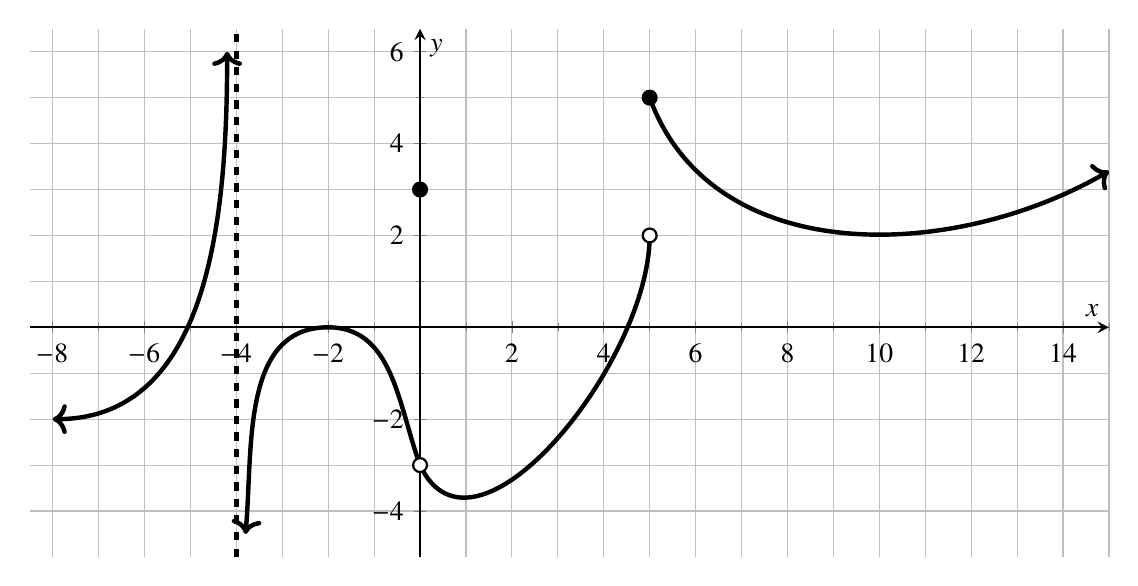
\begin{tikzpicture}[]
%cubic
\begin{axis}[
    scale = 2,
    axis equal image,
    thick, my style, 
    xtick={-8,-6,...,15}, 
    ytick={-4,-2,..., 6},
    xmin=-8.5, xmax=15, 
    ymin=-5, ymax=6.5, 
    minor y tick num=1, 
    minor x tick num=1, 
    mark size=3.0pt, 
    grid = both, 
]
    % Curves
    \draw[ultra thick, <->] (-8, -2) to[out=0, in = -90] (-4.2,6);
    \draw[ultra thick, <-](-3.8, -4.5) to[out = 85, in = -180] (-2, 0) to[out = 0, in = +90+20] (0, -3);
    \draw[ultra thick, -](0, -3) to[out = -65, in = -90] (5, 2);
    \draw[ultra thick, ->](5, 5) to[out = -90+20, in = 180+30] (15, 3.4);
    \draw[ultra thick, dashed] (-4, -5) -- (-4, 8);

    % Hole at (0, -3)
    \draw[fill=white, thick] (0, -3) circle[radius=2.5pt];

    % Hole at (5, 2)
    \draw[fill=white, thick] (5, 2) circle[radius=2.5pt];

    % Solid point at (10, 3)
    \filldraw (0, 3) circle[radius=2.5pt];

    % Solid point at (5, 5)
    \filldraw (5, 5) circle[radius=2.5pt];
\end{axis}
\end{tikzpicture}
\end{center}

\vspace{.3in}

\begin{subproblems}
\begin{multicols}{4}
\item $\ds \lim_{x \to -4^{+}} f(x) =$ \blank{1 cm}
\item $\ds \lim_{x \to -2} f(x) =$ \blank{1 cm}
\item $\ds \lim_{x \to 0} f(x) =$ \blank{1 cm}
\item $\ds \lim_{x \to 5^{-}} f(x) =$ \blank{1 cm}\\

\end{multicols}
%\item List all $x$-values where the derivative $f'(x)$ is not defined. 
%\hrulefill
%\item Estimate $f'(-1)=$\blank{1cm}. \textbf{Explain} how you computed your estimate.
%\vspace{1in}
\item At what $x$-values(s) is the function $f(x)$ {\bf discontinuous}? \hrulefill\\

\item At what $x$-values(s) does $f(x)$ have a {\bf local minimum}? \hrulefill\\

\item The line $y = -2$ is a horizontal asymptote of $f(x)$. Fill in a statement about a limit that corresponds to this fact.
 
\[\lim_{\fbox{\strut\hspace{1cm}}} \fbox{\strut\hspace{1cm}} = \fbox{\strut\hspace{1cm}}\]\\

\item On what interval(s) is $f(x)$ {\bf concave up}? \hrulefill
 \end{subproblems}

\newpage

%%%%%%%%%%%%%%%%% Compute some derivative
\problem{6 points} Compute the following {\bf derivatives}. Show your work
clearly. You do {\bf not} need to simplify your answers.
\begin{subproblems}
%	\item $\ds y = \frac{x^{3.5}-x^2+e^2}{\sqrt{x}}$
%	\vfill
	\item $\ds f(x) = 3x^4 \cos\left(\frac{x^2}{5}\right)$
	\vfill
	$f'(x)=$
	\vfill
%	\item $\ds g(x) = 5 \cot^2 \left( 4x+3 \right)$
% 	\vfill
	\item $\ds h(x) = 5\ln(2) +\frac{x^{2.5}}{\ln(4x^3)}$
	\vfill
	$h'(x)=$
	\vfill
%	\item $(xy)^2 + 3x = y^2$   (You {\bf must} solve for $\ds \frac{dy}{dx}$.)
%	\vfill
\end{subproblems}

%%%% Or generic abs. max/min
\problem{9 points}

Find the {\bf absolute maximum} and the {\bf absolute minimum} of the function $f(x) = x^3 - 3x^2$ on the interval $[-1, 4]$. Justify your answer.
\vfill
\vfill
\vfill
\vfill
\vfill
\vfill
  \begin{flushright}
    {\bf maximum value} of $f(x)$: \underline{\hspace{3cm}} \\
    \vspace{0.3cm}
    {\bf minimum value} of $f(x)$: \underline{\hspace{3cm}}
  \end{flushright}

\newpage

\problem{10 points} A cabbage is launched upward at 40 meters per second
from a cannon that sits 100m above the ground. The height (in meters) of the
cabbage relative to the ground after $t$ seconds is given by the function
$$
h(t) = -5t^2+40t+100
$$
\begin{subproblems}
	\item Determine the velocity of the cabbage after $0.5$ seconds. Include units.
	\vfill
	\item Determine the acceleration of the cabbage at $0.5$ seconds. Include units.
	\vfill
	\item Determine when the cabbage will reach its maximum height. Justify your answer using calculus. Include units.
	\vfill
	\vfill
	%\item Determine how long the cabbage is in the air. Include units.
	%\vfill
	%\item Determine the velocity of the cabbage when it hits the ground. Include units.
	%\vfill
\end{subproblems}

\problem{5 points} Let $h(x) = 1-3\tan(x)$
\begin{subproblems}
	\item Find the linearization $L(x)$ of $h(x)$ near $x=0$.
	\vfill
	\item Use your answer from part (a) to approximate $h(0.1)$.  {\bf Simplify} your answer.
	\vfill
\end{subproblems}

\newpage

\problem{10 points}A blimp is flying in a straight line at a constant altitude of 300 meters towards an observer who is watching from the ground. The blimp is moving horizontally at 40 meters per second. Let \( \theta \) be the angle between the ground and the line of sight from the person to the blimp. (See diagram.)

\begin{center}
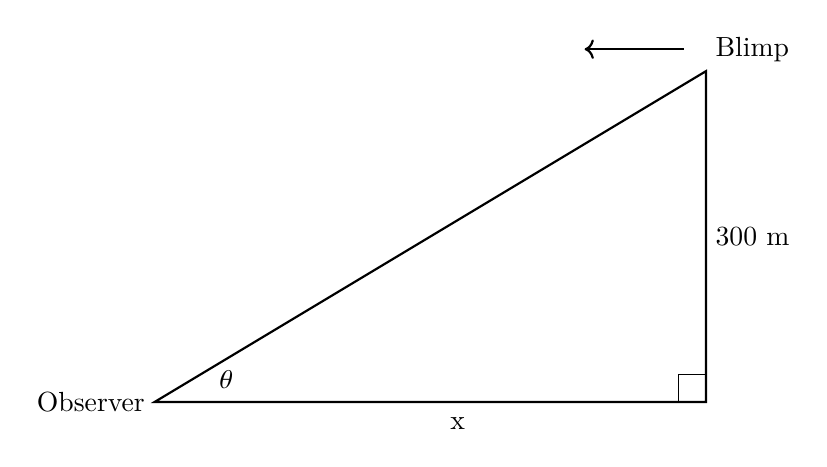
\begin{tikzpicture}[scale=0.07]

  % Coordinates
  \coordinate (A) at (0,0);       % Observer
  \coordinate (B) at (100,0);     % Point under blimp
  \coordinate (C) at (100,60);   % Blimp

  % Triangle
  \draw[thick] (A) -- (B) -- (C) -- cycle;

  % Right angle marker
  \draw (95,0) rectangle +(5,5);

  % Labels
  \node[below] at (55,-1) {x};
  \node[right] at (100,30) {300 m};
  \node[above right] at (100,60) {Blimp};
  \node[left] at (0,0) {Observer};
  \node[right] at (10,4) {$\theta$};
\draw[->, thick] (96,64) -- (78,64);

  % Angle theta
  %\pic [draw, angle radius=30, "$\theta$"] {angle = C--A--B};

\end{tikzpicture}
\end{center}

\subproblem{}   Write an equation that relates the variables $x$ and $\theta$.
\vspace{.8in}
\subproblem{}   Determine how fast is the angle of elevation \( \theta \) changing when the blimp is 400 meters horizontally from the observer? Include units in your answer.
\vfill

\newpage

%%%%%%%%%%%%%%%%% Compute some limits
\problem{12 points} Compute the following {\bf limits}. Show your work clearly. Be
sure to use {\bf proper notation} where appropriate. Solutions without
proper notation will not receive full credit. Indicate any use of
L'H\^{o}pital's Rule with $\overset{h}{=}$
or $\overset{L'H}{=}$ or something similar. (Be sure to verify
explicitly that L'H\^{o}pital's Rule applies!).
\begin{subproblems}
	\item $\ds \lim_{x \rightarrow \infty} \frac{4x}{\sqrt{x^2-1}}$
	\vfill
	\item $\ds \lim_{x \rightarrow \pi} \frac{x-\pi}{\sin(x)}$
	\vfill
	\item $\ds \lim_{x \rightarrow \infty} x^2e^{-x}$
	\vfill
	\item $\ds \lim_{x \rightarrow 0} \frac{e^x}{\cos(x)}$
	\vfill
	%\item $\ds \lim_{x \rightarrow 0^+} x^{1/\sin(x)}$
\end{subproblems}

\newpage

%\problem{8 points}
%The function $G(x)$ is continuous on its domain $(-\infty,0) \cup (0,\infty).$
%\begin{itemize}
%\item $G(0)=4$
%\item $G'(x)$ is positive for all x in the interval $(-\infty,0).$
%\item $G'(x)$ is negative for all x in the interval $(0,\infty).$
%\item $G''(x)$ is positive in the interval $(2, \infty).$
%\item $G''(x)$ is negative in the interval $(-\infty,2)$
%\item $\lim_{x\to\infty} G(x)=0$.
%\end{itemize}
%{\bf Sketch the graph} of $G(x)$. Clearly identify any local maxima, local minima, inflection points and asymptotes in the graph.
%\vfill
%\begin{center}
%\begin{tikzpicture}[scale=1]
%\draw[->] (-6.2,0) -- (6.2,0) node[right] {$x$};
%\draw[->] (0,-6.2) -- (0,6.2) node[left] {$y$};
%\draw[help lines, dashed] (-6.2,-6.2) grid (6.2,6.2);
%\end{tikzpicture}
%\end{center}

%\newpage

%%%%%%%%%%%Integrals
\problem{12 points} Compute the following \emph{integrals and antiderivatives}. Give the most general answer, and show your work. Clearly indicate any substitutions you use.

\begin{subproblems}
	\item $\ds \int_{0}^3 t^2+6t-e^t \: dt$
	\vfill
%	\item  $\ds \int  t^{1/2}\left(2t^{-1/2}-t^{-1}\right) +\ln(2) \: dt$
%	\vfill
%	\item $\ds \int \frac{1}{1+x^{2}} + 1 + x^2  \: dx$
%	\vfill 
	\item $\ds \int \csc(3\theta-\pi/2)\cot(3\theta - \pi/2) \: d\theta $
	\vfill 
	\item $\ds \int \frac{12e^x}{(e^x+12)^3} \: dx $
	\vfill 
\end{subproblems}

 \newpage


%%%%%%%%%%%%%%%%% Net Change + Max Rate of Change - Applied calculus context

\problem{15 points} At 2:00 pm ($t = 0$), the main water line in your apartment bursts. The rate at which water is flowing from the break is given by $\ds r(t)=\frac{5t}{1+t^2}$, where $r$ is measured in gallons per hour and $t$ is measured in hours.% from $t=0$ to $t=24.$
\begin{subproblems}
	\item Find $r(3)$. Write a sentence that someone who has not taken calculus could understand to explain the meaning of $r(3)$. Include units.
	\vfill
	\item Evaluate $\ds \int_1^2 r(t) \: dt$.
	\vfill
	\vfill
	\item Write a sentence that someone who has not taken calculus could understand to explain the meaning of $\ds \int_1^2 r(t) \: dt$. Include units.
	\vfill
	\item At 3:00pm, is the rate of flow increasing, decreasing or staying the same? Explain how you know.%Show work and explain your answer. 
	\vfill
	\vfill
%	\item At what time is the rate of flow of the water at its maximum? Give your answer as a time and justify your answer that your answer is the maximum. %Show some work, and answer the question with a sentence.
%	\vfill
%	\vfill
\end{subproblems}

\newpage


%%%%%%%%%%%%%%%FTC Part 1
\problem{6 points}
The graph of a function $g(x)$ is shown below.
\begin{center}
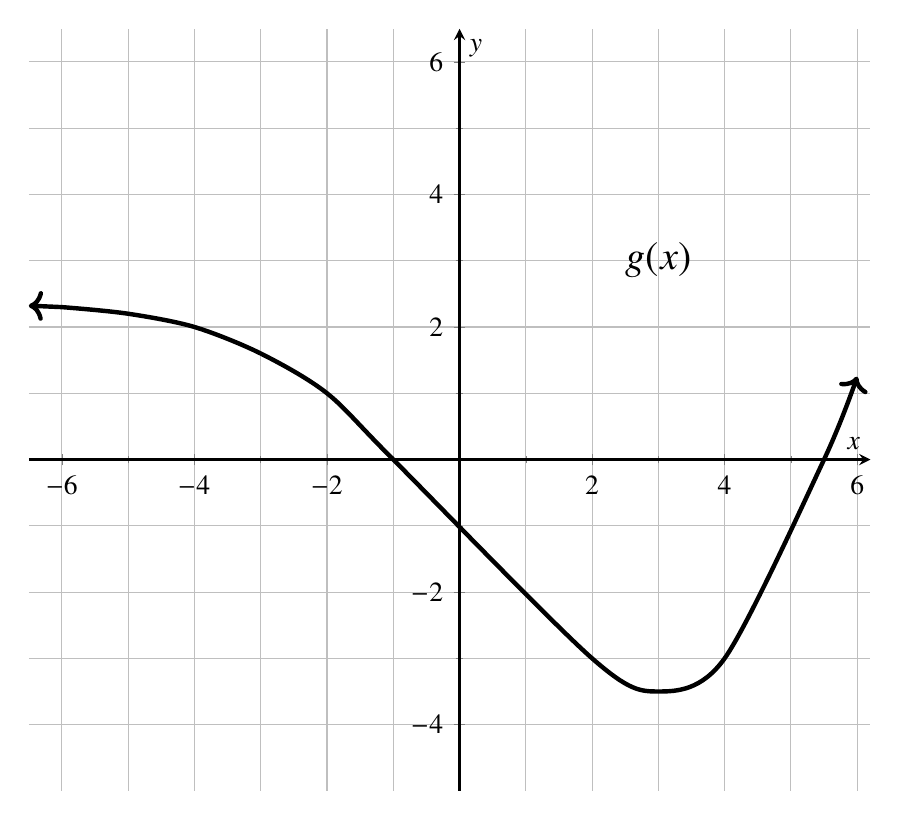
\begin{tikzpicture}[]
%cubic
\begin{axis}[%xscale = 1, yscale = 1, 
scale = 1.7,
axis equal image,
thick, my style, xtick={-8,-6,...,8}, ytick={-4,-2,..., 6},
xmin=-6.5, xmax=6.2, ymin=-5, ymax=6.5, minor y tick num=1, minor x tick num=1, 
mark size=3.0pt, grid = both, ]
\addplot[ultra thick, domain = -5:8, smooth, <->] coordinates{
(-6.5, 2.32)
(-6, 2.3)
(-5, 2.2)
(-4, 2)
(-3, 1.6)
(-2, 1)
(-1,0)
(2, -3)
(3, -3.5)
(4,-3)
(5.5, 0)
(6, 1.25)

};
\path (3,3) node{{\Large $g(x)$}};

\end{axis}


\end{tikzpicture}
\end{center}

Define a new function $\ds A(x) = \int_{-4}^{x} g(t) \ dt$.
\begin{subproblems}
\item Determine $A'(2)$.

\vfill

\item Does $A(x)$ have a local maximum or a local minimum on the interval $(-4, 4)$? If so, state the corresponding $x$-value and explain your answer. If not, explain why not.

\vfill

%\item \emph{Estimate} %$\ds \int_{-5}^{1} f(x) \ dx$ = 
%$A(3) = $\blank{1cm} and clearly explain what calculation you did to arrive at that estimation. (You may want to draw on the graph as part of your explanation.)
%\vfill

\end{subproblems}

\newpage







%% Extra Credit Newton's Method
\fbox{\emph{Extra Credit}} (5 points) A portion of the graph of the function $f(x)=\frac{4}{5}x^5-x-\frac{2}{5}\:$ is shown below.

	\begin{tikzpicture}[yscale=1.8,xscale=3.2]
\draw[->] (-0.5,0) -- (2.2,0) node[right] {$x$};
\draw[->] (0,-2.2) -- (0,2.2) node[above] {$f(x)$};
\draw[help lines, dashed] (-0,2) grid (2,-2);
\foreach \x in {1,2}
\draw (\x,0.1) node[below] {$\x$};
\foreach \y in {-1,1}
\draw (-0.1,\y) node[left] {$\y$};
%\draw[scale=0.5, domain=-3:3, smooth, variable=\x, blue] plot ({\x}, {\x*\x});
	\draw[domain=-0.5:1.4, -, ultra thick,smooth, variable=\x] plot({\x},{0.8*\x^5-\x-0.4});
	\end{tikzpicture}

\begin{enumerate}[a.]%[font = \sffamily,label=\textbf{\alph*}.]
	\item Suppose Newton's method is used to find an approximate solution to
	$f(x)=0$ from an initial guess of $x_0=1$. \emph{Sketch} on the graph how the
	next approximation $x_1$ will be found, \emph{labeling}
	its location on the $x$-axis.
	\vspace{.5in}
	\item If your starting guess is $x_0=1$, \emph{compute} $x_1$. 	\vfill
\end{enumerate}

\vfill

\vfill



\end{document}

%%%%ENDDOCUMENT


